\documentclass[12pt]{article}

\usepackage{booktabs}% http://ctan.org/pkg/booktabs
\usepackage[utf8]{inputenc}
\usepackage{changepage}
\usepackage{pgfplots}
\usepackage{amssymb}
\usepackage{xcolor}
\usepackage{hyperref}
\usepackage{listings}
\usepackage[T1]{fontenc}
\usepackage[utf8]{inputenc}
\usepackage{adjustbox}
\usepackage{amsmath}
\usepackage{mathtools}
\usepackage{biblatex}
\lstset{
  language=Python,
  numbers=left,
  numberstyle=\tiny,
  stepnumber=1,
  numbersep=5pt,
  tabsize=4,
  basicstyle=\ttfamily,
  columns=fullflexible,
  keepspaces,
}
\hypersetup{
    colorlinks,
    citecolor=black,
    filecolor=black,
    linkcolor=black,
    urlcolor=black
}

% Set page size and margins
% Replace `letterpaper' with `a4paper' for UK/EU standard size
\usepackage[letterpaper,top=2cm,bottom=2cm,left=3cm,right=3cm,marginparwidth=1.75cm]{geometry}

% Useful packages
\usepackage{amsmath}
\usepackage{mathtools}
\usepackage{graphicx}
\newenvironment{para}{\begin{adjustwidth}{13mm}{}}{\end{adjustwidth}}

\newcommand\tab[1][1cm]{\hspace*{#1}}

\newcommand{\tabitem}{\llap{\textbullet}}
\newcommand{\Hsquare}{%
\text{\fboxsep=-.2pt\fbox{\rule{0pt}{1ex}\rule{1ex}{0pt}}}%
}

\newtheorem{Definizione}{Definizione}[subsection]
\newtheorem{Lemma}{Lemma}[subsection]
\newtheorem{Teorema/Definizione}{Teorema/Definizione}[subsection]
\newtheorem{Corollario}{Corollario}[subsection]
\newtheorem{Teorema}{Teorema}[subsection]
\newtheorem{Proposizione}{Proposizione}[subsection]
\newtheorem{Notazione}{Notazione}[subsection]
\newtheorem{Commento}{Commento}[subsection]
\newtheorem{Dimostrazione}{Dimostrazione}[subsection]
\newtheorem{Osservazione}{Osservazione}[subsection]
\newtheorem{Nota}{Nota}[subsection]

\title{Basi di dati}
\author{spitfire}
\date{A.A. 2023-2024}
\begin{document}
\begin{figure}
    \centering
    
\includegraphics[width=0.35\textwidth]{Images/Logo scienze bicocca.png}
\end{figure}

\vspace{10cm}
\date{A.A. 2023-2024}


\maketitle

\newpage

\tableofcontents
\newpage
\section{Introduzione}
Una base di dati è un \textbf{insieme organizzato di dati} utilizzati per il supporto allo svolgimento di attività (di un ente, azienda, ufficio, persona).
Facciamo un passo indietro e ricordiamo cos'è invece \textbf{l'informatica}:
essa è la \textbf{scienza del trattamento razionale dell'informazione}, spesso per mezzo di \textbf{macchine automatiche}.
Essa è considerata come supporto alla conoscenza umana e alla comunicazione.
L'informatica ha due anime:
\begin{itemize}
    \item \textbf{Metodologica}: i metodi per la soluzione di problemi e la gestione delle informazioni
    \item \textbf{Tecnologica}: i calcolatori elettronici e i sistemi che li utilizzano
\end{itemize}
\subsection{Sistemi informativi}
Un \textbf{sistema informativo} è un componente (sottosistema) di un'organizzazione che gestisce le informazioni di interesse (cioè utilizzate per il perseguimento degli scopi dell'organizzazione).
Le funzioni di un sistema informativo sono:
\begin{itemize}
    \item \textbf{Acquisizione/memorizzazione}
    \item \textbf{Aggiornamento}
    \item \textbf{Interrogazione}
    \item \textbf{Elaborazione}
\end{itemize}
Il concetto di "sistema informativo" è \textbf{indipendente da qualsiasi automazione}: esistono organizzazioni
la cui ragion d'essere è la \textbf{gestione di informazioni} (es. servizi anagrafici e banche) e che operano da secoli.
Anche prima di essere automatizzati, molti sistemi informativi si sono evoluti verso una \textbf{razionalizzazione e standardizzazione} delle procedure e dell'organizzazione delle informazioni.
\subsection{Sistema informatico}
Un \textbf{sistema informatico} è una porzione \textbf{automatizzata} di un sistema informativo; cioè la parte del sistema informativo che gestisce le informazioni con tecnologia informatica.
\begin{center}
    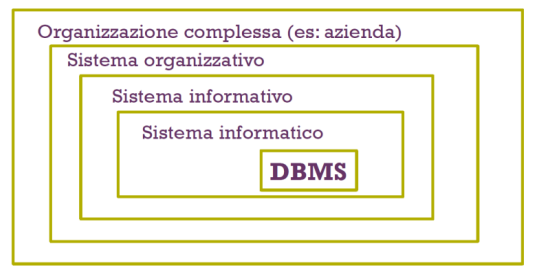
\includegraphics[width = 0.55\textwidth]{Images/1.PNG}
\end{center}
\newpage
\noindent
Un sistema informatico:
\begin{itemize}
    \item Garantisce che i dati siano conservati in modo \textbf{permanente} sui dispositivi di memorizzazione
    \item Permette un \textbf{rapido aggiornamento} dei dati per riflettere rapidamente le loro variazioni
    \item Rende i dati \textbf{accessibili alle interrogazioni} degli utenti
    \item Può essere \textbf{distribuito sul territorio}
\end{itemize}
\subsection{Gestione delle informazioni}
Nelle attività umane, le informazioni vengono gestite (registrate e scambiate) in forme diverse:
\begin{itemize}
    \item \textbf{Idee informali}
    \item \textbf{Linguaggio naturale} (scritto o parlato, formale o colloquiale, in una lingua o in un'altra)
    \item \textbf{Disegni, grafici e schemi}
    \item \textbf{Numeri e codici}
\end{itemize}
E su vari supporti, come la memoria umana, su carta o su dispositivi elettronici.
Nelle attività standardizzate dei sistemi informativi complessi, sono state introdotte col tempo forme di organizzazione e codifica delle informazioni via via più precise (e in un certo senso artificiali).
Ad esempio, nei servizi anagrafici si è iniziato con registrazioni discorsive per poi evolversi in registrazioni più complete.
\subsection{Informazioni e dati}
Nei sistemi informatici (e non solo), le \textbf{informazioni} vengono rappresentate in modo essenziale, spartano: attraverso i \textbf{dati}.
Diamo delle definizioni semantiche:
\begin{itemize}
    \item \textbf{Informazione}: notizia, dato o elemento che consente di avere conoscenza più o meno esatta di fatti, situazioni, modi di essere.
    \item \textbf{Dato}: ciò che è immediatamente presente alla conoscenza, prima di ogni elaborazione; (in informatica) elementi di informazione costituiti da simboli che debbono essere elaborati
\end{itemize}
I dati quindi hanno bisogno di essere interpretati!
\subsubsection{Perché i dati?}
La rappresentazione precisa di forme più ricche di informazione e conoscenza è difficile.
I dati costituiscono spesso una risorsa strategica, perché più stabili nel tempo di altri componenti (processi, tecnologie, ruoli, umani).
I dati rimangono gli stessi nella \textbf{migrazione} da un sistema al successivo.
\subsection{Basi di Dati e introduzione ai Database Management Systems (DBMS)}
Come già detto, una \textbf{base di dati} (DB) è una collezione di dati utilizzati per rappresentare le informazioni di interesse in un sistema informativo.
Un \textbf{Database Management System} (DBMS) è invece un \textbf{sistema software} capace di gestire collezioni di dati che siano \textit{grandi, condivise e persistenti}, assicurando la loro \textit{affidabilità e privatezza}.
Possiamo quindi dare due accezioni al termine \textbf{base di dati}:
\begin{itemize}
    \item \textbf{Metodologica}: insieme organizzato di dati utilizzati per il supporto allo svolgimento delle attività di un ente
    \item \textbf{Specifica, metodologica e tecnologica}: Insieme di dati gestito da un DBMS
\end{itemize}
Possiamo dare ancora una definizione: una \textbf{base di dati} è un insieme di archivi in cui ogni dato è rappresentato logicamente
una sola volta e può essere utilizzato da un insieme di applicazioni o da diversi utenti secondo opportuni criteri di riservatezza.
\begin{center}
    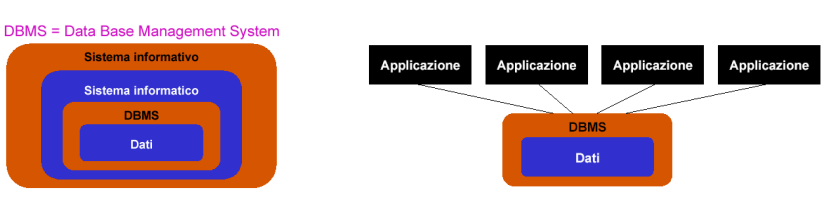
\includegraphics[width = 1\textwidth]{Images/2.PNG}
\end{center}
Le caratteristiche di una base di dati sono:
\begin{itemize}
    \item I dati sono \textbf{molti}
    \item I dati hanno un \textbf{formato definito}
    \item I dati sono \textbf{permanenti}
    \item I dati sono \textbf{raggruppati} per insiemi \textbf{omogenei} di dati
    \item Esistono \textbf{relazioni specifiche} tra gli insiemi di dati
    \item La ridondanza è \textbf{minima e controllata}: è assicurata la consistenza delle informazioni
    \item I dati sono disponibili \textbf{per utenze diverse e concorrenti}
    \item I dati sono \textbf{controllati}: protetti da malfunzionamenti hardware e software
    \item I dati della base di dati sono \textbf{indipendenti dai dati di un qualsiasi programma}
\end{itemize}
\subsection{Database Management System}
Un DBMS è un insieme di programmi che permettono di creare, usare e gestire una base di dati.
Quindi un DBMS è un sistema software general purpose che facilita il processo di \textbf{definizione, costruzione e manipolazione} del database per varie applicazioni.
Vi sono 3 fasi nella \textbf{creazione di un database}:
\begin{enumerate}
    \item \textbf{Definizione}
    \item \textbf{Creazione/Popolazione}
    \item \textbf{Manipolazione}
\end{enumerate}
Una volta creato un database, si potranno effettuare su di esso delle \textbf{interrogazioni} (queries).
L'efficacia delle queries dipende da:
\begin{itemize}
    \item Conoscenza dle contenuto del DB
    \item Esperienza con il linguaggio di interrogazione
    \item Semplicità ed efficacia dell'interfaccia di interrogazione
\end{itemize}
Un DBMS è quindi un \textbf{sistema} che gestisce collezioni di dati:
\begin{itemize}
    \item \textbf{Grandi}
    \item \textbf{Persistenti}
    \item \textbf{Condivise}
\end{itemize}
garantendo:
\begin{itemize}
    \item \textbf{Privatezza}
    \item \textbf{Affidabilità}
    \item \textbf{Efficienza}
    \item \textbf{Efficacia}
\end{itemize}
\subsection{Caratteristiche delle basi di dati}
Le basi di dato sono:
\begin{itemize}
    \item \textbf{Grandi}: dimensioni (molto) maggiori della memoria centrale dei sistemi di calcolo utilizzati. Il limite deve essere solo quello fisico dei dispositivi
    \item \textbf{Persistenti}: hanno un tempo di vita indipendente dalle singole esecuzioni dei programmi che le utilizzano
    \item \textbf{Condivise}: Ogni organizzazione (specie se grande) è divisa in settori o comunque svolge diverse attività. Ciascun settore/attività ha un (sotto)sistema informativo (non necessariamente disgiunto)
    \item I possibili problemi sono la \textbf{ridondanza}, cioè la ripetizione di informazioni, e \textbf{l'incoerenza}, cioè le varie versioni della basi di dati potrebbero non coincidere
\end{itemize}
\subsection{Archivi e basi di dati}
\begin{center}
    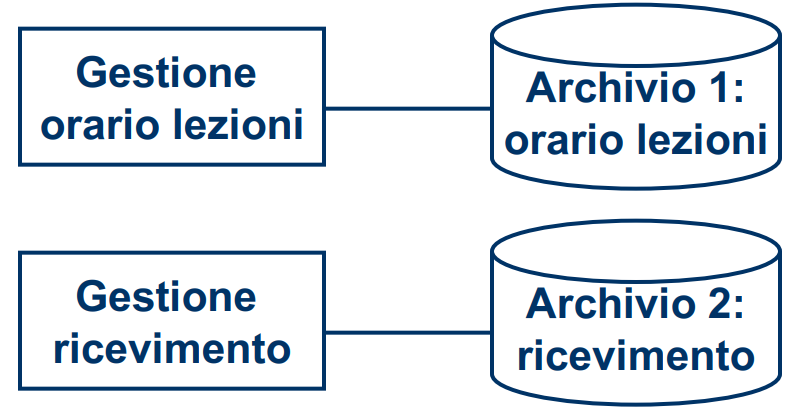
\includegraphics[width = 0.55\textwidth]{Images/3.PNG}
\end{center}
\begin{center}
    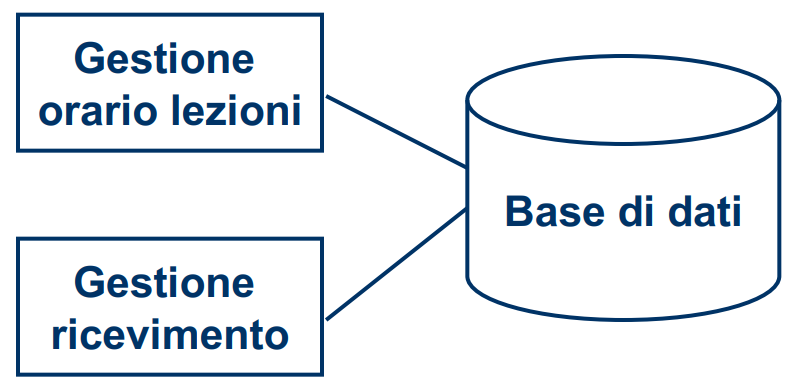
\includegraphics[width = 0.55\textwidth]{Images/4.PNG}
\end{center}
\subsection{Condivisione delle basi di dati}
Una base di dati è una risorsa \textbf{integrata e condivisa} fra applicazioni.
Diventa quindi possibile svolgere attività diverse su dati condivisi: sono necessari quindi \textbf{meccanismi di autorizzazione}.
Diventano anche possibili accessi di più utenti ai dati condivisi: sono quindi necessarie politiche e meccanismi di controllo della \textbf{concorrenza}.
\subsection{Caratteristiche dei DBMS}
I DBMS garantiscono \textbf{privatezza}; cioè si possono definire meccanismi di autorizzazione: l'utente A è, per esempio, autorizzato a leggere tutti i dati e a modificare quelli sul ricevimento; tuttavia
l'utente B è magari autorizzato a leggere i dati di X e a modificare i dati di Y. \newline
I DBMS garantiscono inoltre \textbf{l'affidabilità} dei dati, cioè la resistenza a malfunzionamenti hardware e software.
Per implementare questa caratteristica è quindi fondamentale \textbf{gestire le transazioni}.
\subsection{Transazioni}
Le \textbf{transazioni} sono l'insieme di operazioni da considerare indivisibili ("\textbf{atomiche}"), corrette anche in presenza di \textbf{concorrenza} e con effetti \textbf{definitivi}.
La sequenza di operazioni sulla base di dati viene eseguita per intero o per niente: per esempio, il trasferimento di fondi da un conto A ad un conto B avviene o tramite il prelevamento da A e il versamento su B o niente affatto.
L'effetto di transazioni concorrenti deve essere \textbf{coerente} (ad esempio "equivalente" all'esecuzione separata delle richieste concorrenti): per esempio, se due assegni emessi sullo stesso conto corrente vengono incassati \textbf{contemporaneamente},
si deve evitare di trascurarne uno.
La conclusione positiva di una transazione corrisponde ad un impegno (in inglese \textbf{commit}) a mantenere traccia del risultato in modo definitivo, anche in presenza di guasti e di esecuzione concorrente.
\subsection{Caratteristiche dei DBMS}
I DBMS devono essere \textbf{efficienti}, cioè devono cercare di utilizzare al meglio le risorse di spazio di memoria (principale e secondaria) e di tempo (di esecuzione e di risposta).
I DBMS, con tante funzioni, rischiano l'inefficienza e per questo ci sono grandi investimenti e competizione. L'efficienza è anche il risultato della qualità delle applicazioni. \newline
I DBMS devono essere \textbf{efficaci}, cioè devono cercare di rendere produttive le attività dei loro utilizzatori, offrendo funzionalità articolare, potenti e flessibili.
\subsection{Descrizioni dei dati nei DBMS}
Descrizioni e rappresentazione dei dati a livelli diversi permettono \textbf{l'indipendenza dei dati} dalla rappresentazione fisica: i programmi fanno riferimento alla struttura a livello più altro, e le rappresentazione sottostanti possono essere modificate senza necessità di modificare i programmi.
Possiamo precisare questo concetto attraverso il concetto di \textbf{modello dei dati}
\subsubsection{Modello dei dati}
Il \textbf{modello dei dati} è l'insieme di costrutti utilizzati per organizzare i dati di interesse e descriverne la dinamica.
Esso ha una componente fondamentale: i \textbf{meccanismi di strutturazione} (o \textbf{costruttori di tipo}): come nei linguaggi di programmazione
esistono meccanismi che permettono di definire nuovi tipi, così ogni modello dei dati prevede alcuni costruttori.
Ad esempio, il \textbf{modello relazionale} prevede il costruttore \textbf{relazione}, che permette di definire insiemi di record omogenei.
\subsection{Schema e istanza della base di dati}
\begin{center}
    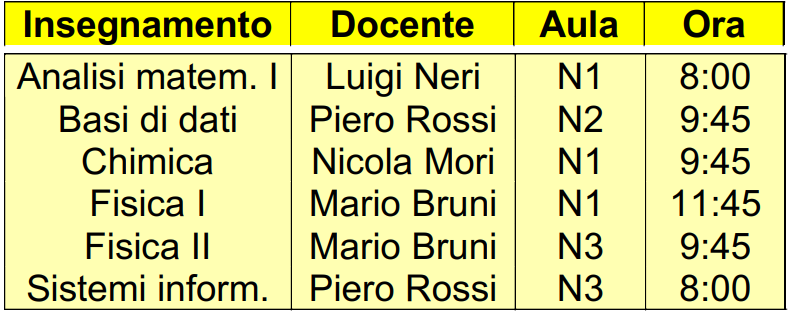
\includegraphics[width = 0.60\textwidth]{Images/5.PNG}
\end{center}
In ogni base di dati esistono:
\begin{itemize}
    \item Lo \textbf{schema}, sostanzialmente invariante nel tempo, che ne descriva la struttura e il significato (aspetto intensionale; es. le intestazioni delle tabelle). Lo schema quindi costituisce l'aspetto \textbf{intensionale}, ovvero la descrizione "astratta" delle proprietà, ed è invariante nel tempo
    \item \textbf{L'istanza}, i valori attuali, che possono cambiare anche molto rapidamente (aspetto estensionale; es. il "corpo" di ciascuna tabella). L'istanza quindi costituisce invece l'aspetto \textbf{estensionale} "concreto", che varia nel tempo al variare della situazione di ciò che stiamo descrivendo
\end{itemize}
\subsection{Modello dei dati logico}
I modelli dei dati logici sono adottati nei DBMS esistenti per l'organizzazione dei dati:
\begin{itemize}
    \item utilizzati dai programmi
    \item indipendenti dalle strutture fisiche
\end{itemize}
Esempi di essi sono il modello \textbf{relazionale}, reticolare, gerarchico, a oggetti, XML, ...
\subsubsection{Modello relazionale}
Nel modello relazionale i dati vengono strutturati in tabelle, in particolare un DBMS relazionale può essere pensato come un insieme di tabelle.
Ogni tabella mantiene informazioni di tipo omogeneo. Diverse tabelle sono collegate (in relazione) fra loro grazie alla presenza di un \textbf{campo comune}, che permette di mettere in relazione i dati delle due tabelle.
Nel modello relazionale:
\begin{itemize}
    \item \textbf{Lo schema} è la descrizione della struttura delle tabelle (stabile nel tempo)
    \item \textbf{L'istanza} sono i valori dei campi della tabella
\end{itemize}
\begin{center}
    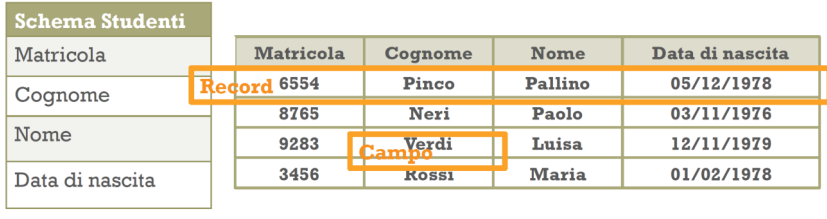
\includegraphics[width = 0.85\textwidth]{Images/6.PNG}
\end{center}
\subsection{Modello dei dati concettuale}
I modelli dei dati concettuali permettono di rappresentare i dati in modo indipendente da ogni sistema.
\begin{itemize}
    \item cercando di descrivere i concetti del mondo reale
    \item sono utilizzati nelle fasi preliminare di progettazione (quali informazioni sono utili? Come sono collegate?)
\end{itemize}
Il più diffuso è il modello \textbf{Entity-Relationship}
\newpage
\subsection{Architettura di un DBMS}
Possiamo strutturare l'architettura di un DBMS in maniera \textbf{semplificata} nel seguente modo:
\begin{center}
    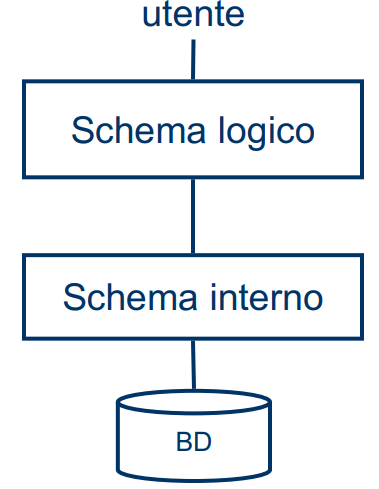
\includegraphics[width = 0.35\textwidth]{Images/7.PNG}
\end{center}
Nella quale:
\begin{itemize}
    \item \textbf{Schema logico}: descrizione della base di dati nel modello logico (ad esempio, la struttura della tabella)
    \item \textbf{Schema interno (o fisico)}: rappresentazione dello schema logico per mezzo di strutture di memorizzazione (file ad esempio, ma anche record con puntatori, ordinati in un certo modo)
\end{itemize}
Una delle architetture standard di riferimento per i DBMS è \textbf{L'architettura \newline ANSI/SPARC a tre livelli}:
\begin{center}
    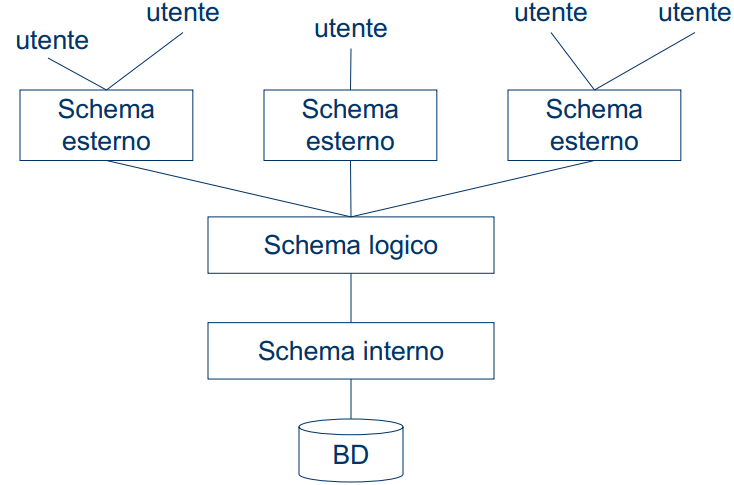
\includegraphics[width = 0.65\textwidth]{Images/8.PNG}
\end{center}
Nella quale:
\begin{itemize}
    \item \textbf{Schema logico}; descrizione dell'intera base di dati nel modello logico "principale" del DBMS
    \item \textbf{Schema fisico}: rappresentazione dello schema logico per mezzo di strutture fisiche di memorizzazione
    \item \textbf{Schema esterno}: descrizione di parte della base di dati in un modello logico ("viste" parziali, derivate, anche in modelli diversi)
\end{itemize}
\begin{center}
    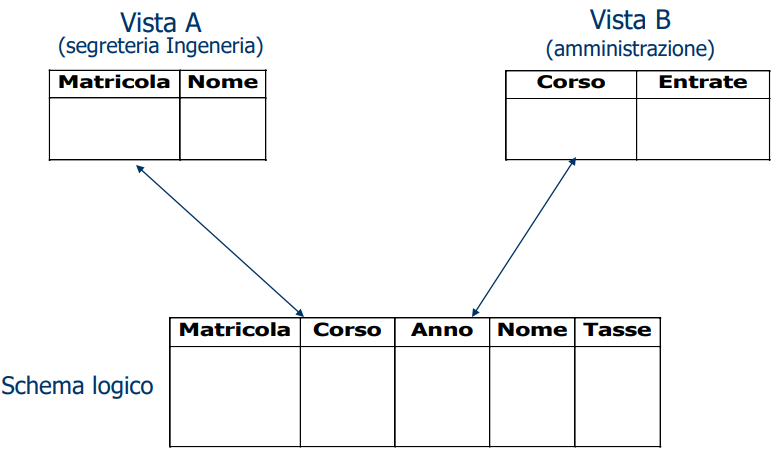
\includegraphics[width = 0.75\textwidth]{Images/9.PNG}
\end{center}
\subsection{Indipendenza dei dati}
Il livello logico è indipendente da quello fisico: una tabella è utilizzata nello stesso modo qualunque sia la sua realizzazione fisica (che può anche cambiare nel tempo).
In questo corso vedremo solo il livello logico e non quello fisico.
La conseguenza della articolazioni in livelli è che l'accesso avviene solo tramite il \textbf{livello esterno} (che può coincidere con il livello logico).
Vi sono due forme di indipendenza:
\begin{itemize}
    \item \textbf{Indipendenza fisica}
    \item \textbf{Indipendenza logica}
\end{itemize}
\subsubsection{Indipendenza fisica}
Il livello logico e quello esterno sono indipendenti da quello fisico. Una relazione è utilizzata nello stesso modo qualunque sia la sua realizzazione fisica.
La realizzazione fisica può cambiare senza che debbano essere modificati i programmi che usano la base di dati.
\subsubsection{Indipendenza logica}
Il livello esterno è indipendente da quello logico. Aggiunte o modifiche alle viste non richiedono modifiche al livello logico.
Le modifiche allo schema logico che lasciano inalterato lo schema esterno sono quindi \textbf{trasparenti}.
\subsection{Linguaggi per basi di dati}
Vi sono due tipi di linguaggi per le basi di dati:
\begin{itemize}
    \item \textbf{Data Definition Languages}(DDL): Servono a definire degli schemi logici, fisici e delle autorizzazioni di accesso
    \item \textbf{Data Manipulation Languages}(DML): Servono per effettuare l'interrogazione e l'aggiornamento delle basi di dati 
\end{itemize}
Alcuni linguaggi come SQL (Structured Query Language) hanno funzioni di entrambe le categorie.
\subsection{Personaggi e interpreti}
Si possono identificare diverse figure durante l'intero ciclo di vita di una base di dati:
\begin{itemize}
    \item \textbf{Progettisti} e realizzatori di \textbf{DBMS}
    \item \textbf{Progettisti della base di dati} e amministratori della base di dati (\textbf{DBA})
    \item \textbf{Progettisti} e programatori di \textbf{Applicazioni}
    \item \textbf{Utenti}
    \begin{itemize}
        \item Utenti \textbf{finali}(terminalisti): eseguono applicazioni predefinite(\textbf{transazioni})
        \item Utenti \textbf{casuali}: eseguono operazioni non previste a priori, usando linguaggi interattivi
    \end{itemize}
\end{itemize}
\subsubsection{Database administrator (DBA)}
Un \textbf{database administrator}(DBA) è una persona o gruppo di persone responsabile del controllo centralizzato e della gestione del sistema, delle prestazioni, dell'affidabilità e delle autorizzazioni.
Le funzioni del DBA includono quelle di progettazione, anche se in progetti complessi ci possono essere distinzioni.
\subsubsection{Utenti del DBMS}
\begin{center}
    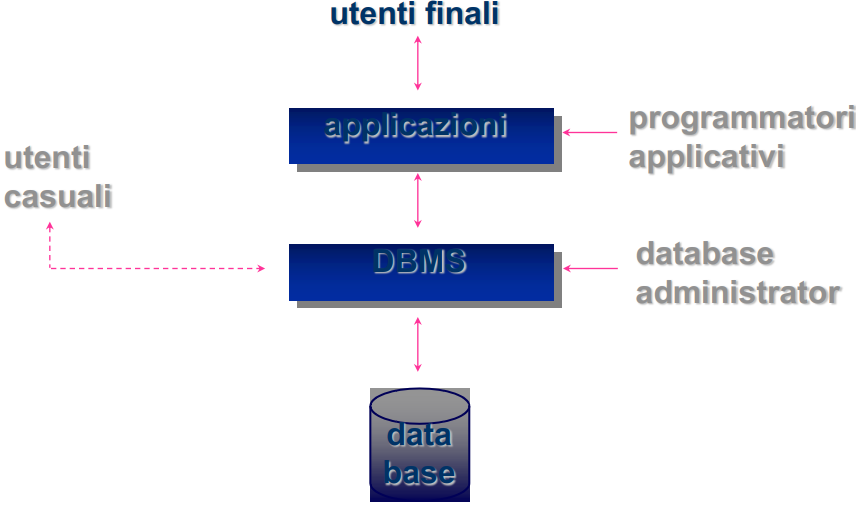
\includegraphics[width = 0.75\textwidth]{Images/10.PNG}
\end{center}
\subsection{Vantaggi e svantaggi dei DBMS}
Vediamo quali sono i \textbf{vantaggi} di avere un DBMS:
\begin{itemize}
    \item Permettono di considerare i dati come risorsa comune di un'organizzazione, a disposizione di molteplici applicazioni e utenti
    \item Offrono un modello della parte di mondo di interesse che è unificato e preciso, utilizzabile in applicazioni attuali e future
    \item Offrono un controllo centralizzato dei dati, riducendo ridondanze e inconsistenze
    \item Permettono l'indipendenza dei dati: favoriscono lo sviluppo di applicazioni flessibili e facilmente modificabili
\end{itemize}
Vediamo quali sono invece gli \textbf{svantaggi} di avere un DBMS:
\begin{itemize}
    \item Un DBMS è costoso, complesso e ha specifici requisiti in termini di software e hardware
    \item Diventa difficile separare, tra tutti i servizi offerti da un DBMS, quelli effettivamente usati da quelli inutili
    \item Sono inadatti alla gestione di applicazioni con pochi utenti (NB: Dipende dai costi operativi)
\end{itemize}
\subsection{Caratteristiche dell'approccio con basi di dati}
L'approccio alla \textbf{rappresentazione dei dati tramite basi di dati} ha le seguenti caratteristiche:
\begin{itemize}
    \item \textbf{Astrazione dei dati}: si usa un \textbf{modello dati} per nascondere dettagli e presentare all'utente una \textit{vista concettuale} del database
    \item \textbf{Supporto di viste multiple dei dati}: Ogni utente può usare una vista (view) differente del database, contente solo i dati di interesse per quell'utente
\end{itemize}

\end{document}